\section{Technologies Used}

This section presents an overview of the key technologies used and
their place in the PaWS framework: Tpips, Python, Pylons, Virtual
Environment and Web application technologies (Javascript, Ajax and
JQuery).

\subsection{Tpips}
\label{tpips_interface}

\emph{Tpips} is the line interface and scripting language of the PIPS
project. It allows to use all of PIPS functions in an easy and
user-friendly way, because it simplifies usage of database when
performing operations, it handles all accesses to database, for
instance itself.  Due to using PIPS metavariables, such as \%ALL,
Tpips enables the application of PIPS commands to several modules with
one command. Another advantage of this interface is that it provides
on-line help and automatic completion. Tpips is a great tool for all
tasks which are repeatable and do not require any interaction with the
user.

In the PAWS project, the Tpips interface is used to implement the demo
mode. 
A fixed Tpips script, with a fixed set of PIPS passes, is applied to a
given source file, potentially modified by the user.
%On
%source file, even if it was modified by user, there is Tpips script
%performed with prepared, always the same set of well-known
%operations. 
That allows PaWS to separate the indivudual steps and their
results. They are shown to the user one by one. Also a Tpips script may be
more understandable for new user than Python PyPS code.

\subsection{Python}
\label{python_description}

Python is a portable\footnote{It runs on Windows, Linux/Unix, Mac OS
  and has been ported to the Java and .NET virtual machines} script
programming language. Python is one of the most commonly used
procedural programming languages because of the clearness of its syntax,
its intuitive object orientation, its extensibility provided by modularity -
modules can be written not only in Python but even in C or Java - and its
very high level dynamic data types. One of the major advantages of
Python language is its ability of being used by applications as a
scripting interface.  There is also a lot of tools based on this
language. They are easy to integrate and to extend. It was the main
advantage of using the Pylons Project\cite{pylons} - WEB application
framework technology based on Python. Due to that, PyPS, PIPS Python
interface, could be easily linked to WEB technologies.

\begin{figure}[h!]
  \centering
  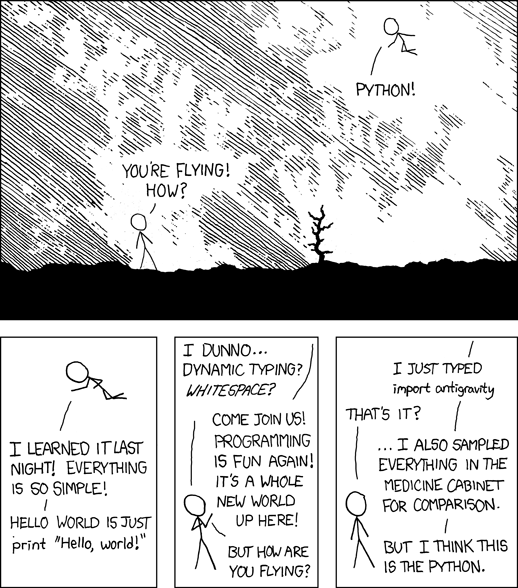
\includegraphics[width=0.6\textwidth]{reportCh2/python}
  \caption{Python by xkcd\cite{python_xkcd}}
  \label{fig:python}
\end{figure}

\subsection{Virtual Environment}
\label{virtualenv}

Virtualenv\cite{virtualenvlit} is the tool used to create isolated
Python environments. Thanks to that, it is possible to make several
distinct environments, which share the same version of Python, but can
have different sets of modules, libraries and packages. All of them
are installed in the Python \emph{site-packages} directory.

This tool is protecting applications against conflicts caused by
different requirements.

\subsection{Pylons}
\label{pylons_descriptions}

Pylons \cite{pylons} is a flexible Python framework based on the
MVC\footnote{MVC stands for \emph{Model-View-Controller}, more in
  section \ref{mvc}} design pattern and WSGI\footnote{WSGI\cite{wsgi}
  stands for \emph{Web Server Gateway Interface} and it is the Python
  standard which specifies interface between web servers and web
  applications.} pattern. Besides its basic WEB application server
functions, Pylons provides also a set of tools and libraries which
extend its way of working, but it does not impose the specific
solutions nor the tools that should be used. The developped can decide
which modules he/she wants to include in his/her application. This
approach guarantees that the application consists only of the
necessary modules and is as light as possible. If it is necessary,
adding third-party libraries is also very easy and intuitive. This
possibility of choosing, adding and composing modules makes Pylons
a very flexible and light framework. It is also very easy to learn and
to use by new developpers.

As written above, Pylons provides a lot of tools which simplify the
development of a WEB application. One of main ones, the
Routes\cite{routes} framework, generates and maps URL addresses to
code. Another tool, WebHelpers\cite{webhelpers} is a set of utility
functions for generating JavaScript\cite{javascript} code. To create
HTML code combined with Python and to pass variables to them, Pylons
is using a \emph{templating system}. It allows user to write HTML and
embed Python code when it is needed\cite{templating_system}. This
solution also supports reusability of the code. The default templating
language is Mako\cite{mako}.

Pylons also can operate on databases, using \emph{Object Relational
  Managers} such as SQLAlchemy\cite{sqlalchemy} or
SQLObject\cite{sqlobject}). In addition it provides caching mechanisms
and manages session variables.

\subsection{Web Application Technologies}
\label{web_application_technologies}

Interactions between users and server are handled by Ajax\cite{ajax}
(Asynchronous JavaScript and XML). Thanks to that technology, the user
view can be refreshed without reloading the whole document. It is
performed in an asynchronous way, which enables user to execute other
operations at the same time. Ajax technology is built in Pylons.


Ajax is used also by JQuery\cite{jquery}, a light and fast library
that contains tools to use Javascript in more advanced ways like
animations or dynamic modifications of site content. Changes provided
by JQuery do not require modifications of the HTML code of the site,
which is important for the developper.

\subsection{Other Tools}
\label{other_technologies}

\begin{itemize}

\item {\bf Pygments}\cite{pygments} is a Python syntax highlighting
  library. It supports a significant number of languages and markup
  formats. There is also a mechanism which allows the developper to
  define his/her own parser to recognize user specific
  languages. Pygments can be used as a library or as a command-line
  tool.

\item {\bf Pyrops} is a Python module based on {\bf pyro}, PYthon
  Remote Objects\cite{pyro}. Pyrops was created as a solution for the
  problem of concurrent accesses to Pips workspaces - it was not
  possible to work on several workspaces at the same time in a
  script\cite{pyps_doc}. Pyrops encapsulate each workspace in a new,
  separate program in a transparent way\footnote{Transparency is
    provided by RPC (and by pyro)\cite{pyps_pass_manager}}. Usage of
  Pyrops is easy for Pyps user - Pyrops workspace inherites of Pyps
  workspace and they are used in the same way.

\item {\bf GCC}\cite{gcc} - the GNU Compiler Collection is one of
  the most popular compiler for C and C++ languages. In PaWS, GCC is
  used for checking the correctness of the user input before performing
  PIPS operations.

\item {\bf F77}\cite{fortran77} and {\bf gFortran}\cite{gfortran} are
  Fortran compilers. They are used in PaWS for the same reason as GCC
  - to check input source code before PIPS is involved.

\item {\bf Fabric}\cite{fabric} - a Python library for automatic
  deployment and setting up of the application. It can be used as a
  library but also as command-line tool. The application developper
  must provide a requirement file where all the dependencies of the
  application and its versions are described. A second file must be
  supplied. It is called \emph{fabfile.py}. It specifies all the
  operations (like setup, installation, clean etc.) that can be used.

%%  \item {\bf versioning}
%%   ??

\end{itemize}



